\documentclass{scrartcl}
\usepackage{dominatrix}
\usepackage{tikz}
\usepackage{pgfplots}
\pgfplotsset{
  every axis/.append style={font=\small},
  compat=newest
}

\begin{document}
  \begin{framed}
  CS 5220 Introduction to Parallel Programming \hfill Fall 2015 \\
  Kenneth Lim (\href{mailto:kl545@cornell.edu}{kl545}), Scott Wu (\href{mailto:ssw74@cornell.edu}{ssw74}), Robert Chiodi (\href{mailto:rmc298@cornell.edu}{rmc298}), Ravi Patel (\href{mailto:rgp62@cornell.edu}{rgp62})  \hfill Final Project \hspace{-3ex}
  \end{framed}
  
  
  \section{Introduction}
  
  \subsection{Smooth Particle Hydrodynamics (SPH)}
  
  \subsection{Code Bases}
  \subsubsection{C Code}
  
  
  \subsubsection{Fortran Code}
    The Fortran code is based off of an SPH code used by Professor Bindel in the spring of 2014 for CS 5220: Applications of Parallel Computers. This code was selected because it directly referenced the solution of the relevant equation (Navier-Stokes) and discussed treatments required to have a working code. SPH can be very unstable without sufficient parameter tuning and having the reference code available allowed easier creation of a serial program that could then be parallelized. Several modifications and additions have been made to this code, as well as it being transferred to Fortran, that will be discussed later. The main contributions taken from the reference code were the leap-frog time integration scheme, handling of walls via damping coefficients, and the recalculation of mass during initialization to have particle densities near the particle reference density. The additions and transfer to Fortran for the serial code led to an order of magnitude speed up for the dam break problem created in the C version using the ``box indicator''. 
    
    The initialization of the Fortran code is handled via an initial text file generated with a python script. This text file contains the number of particles, the time step, the size of the particles, domain side length (with the domain being assumed cubic), frequency of visualization file output, final desired simulation time, and initial position and velocity of all particles. This is a very flexible format for initialization that allows easy rerunning of simulation conditions and the creation of a diverse problem set.
    
    \subsection{Writing of Visualization Files}
    The writing of visualization files is handled the same way in each code. At a specified frequency, by a certain number of time steps in the C version or an amount of simulated time in the Fortran version, a text file is written that contains the number of particles along with their position and velocity. The text files are numbered sequentially with integer tags in order to keep the proper time sequence. A python script we wrote, based loosely off of the visualizer script written for the wave-equation assignment, then plots each particle as a point on a 3D scatter plot and encodes the images together with \texttt{ffmpeg}.
    
  \section{Profiling and Serial Optimization}  
  \subsection{C Code}

  \subsubsection{Profiling}
  
  \subsubsection{Optimizations}
  \subsubsection{Compiler Flags}
  
  \subsection{Fortran Code}
  \subsubsection{Profiling}
  
  \subsubsection{Optimizations}
  \subsubsection{Compiler Flags}
  
  
  \section{Parallelization}
  \subsection{C Code}  
  \subsubsection{OpenMP}
  \begin{table}
  	\begin{tabular}{| c | c | c | c | c | c | c | c |}
  		\hline
  	Case & \# Particles & LLC ($x$,$y$,$z$) & URC ($x$,$y$,$z$) & \# Threads & Time (s) & SS & SSE \\ \hline
	1 & 34,328 & (0.0, 0.0, 0.0) & (0.5, 0.5, 0.5) & 1 & & & \\ \hline		  		
	2 & 34,328 & (0.0, 0.0, 0.0) & (0.5, 0.5, 0.5) & 2 & & & \\ \hline		  		
	3 & 34,328 & (0.0, 0.0, 0.0) & (0.5, 0.5, 0.5) & 4 & & & \\ \hline		  		
	4 & 34,328 & (0.0, 0.0, 0.0) & (0.5, 0.5, 0.5) & 8 & & & \\ \hline		  		
	5 & 34,328 & (0.0, 0.0, 0.0) & (0.5, 0.5, 0.5) & 12 & & & \\ \hline		  		
	6 & 34,328 & (0.0, 0.0, 0.0) & (0.5, 0.5, 0.5) & 16 & & & \\ \hline		  		
	7 & 34,328 & (0.0, 0.0, 0.0) & (0.5, 0.5, 0.5) & 24 & & & \\ \hline		  		
	\end{tabular}
	\caption{Configuration of dam break simulations used for strong scaling study. LLC = Lower Left Corner, URC = Upper Right Corner, SS = Strong Scaling, SSE = Strong Scaling Efficiency.}
	\label{tab:ss}
  \end{table}
  
    \begin{table}
    	\begin{tabular}{| c | c | c | c | c | c | c | c |}
    		\hline
    		Case & \# Particles & LLC ($x$,$y$,$z$) & URC ($x$,$y$,$z$) & \# Threads & Time (s) & SS& SSE \\ \hline
    		1 & 2,197 & (0.0, 0.0, 0.0) & (0.5, 0.5, 0.5) & 1 & & & \\ \hline		  		
    		2 & 4,394 & (0.0, 0.0, 0.0) & (0.5, 0.5, 0.5) & 2 & & & \\ \hline		  		
    		3 & 8,788 & (0.0, 0.0, 0.0) & (0.5, 0.5, 0.5) & 4 & & & \\ \hline		  		
    		4 & 17,576 & (0.0, 0.0, 0.0) & (0.5, 0.5, 0.5) & 8 & & & \\ \hline		  		
    		5 & 26,364 & (0.0, 0.0, 0.0) & (0.5, 0.5, 0.5) & 12 & & & \\ \hline		  		
    		6 & 35,152 & (0.0, 0.0, 0.0) & (0.5, 0.5, 0.5) & 16 & & & \\ \hline		  		
    		7 & 52,728 & (0.0, 0.0, 0.0) & (0.5, 0.5, 0.5) & 24 & & & \\ \hline		  		
    	\end{tabular}
    	\caption{Configuration of dam break simulations used for weak scaling study. LLC = Lower Left Corner, URC = Upper Right Corner, SS = Strong Scaling, SSE = Strong Scaling Efficiency.}
    	\label{tab:ws}
    \end{table}
  
    \textbf{Strong Scaling:}
    
    \textbf{Weak Scaling:}
    
  \subsubsection{Cilk}
  \textbf{Strong Scaling:}
  
  \textbf{Weak Scaling:}
  \subsection{Fortran Code}    
  
  \subsubsection{OpenMP}
  \textbf{Strong Scaling:}
  \begin{figure}
  	\begin{center}
	  	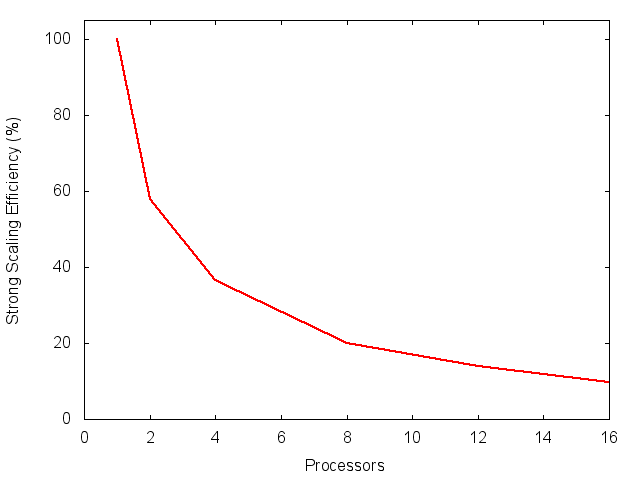
\includegraphics[width=0.7\columnwidth]{./fort_scaling/ss.png}
	  	\caption{Strong scaling for simulations in Table~\ref{tab:ss} using the Fortran code parallelized with OpenMP.}
		\label{fig:ss_fort_omp}
  	\end{center}
  \end{figure}
  
  
  \textbf{Weak Scaling:}  
    \begin{figure}
    	\begin{center}
    		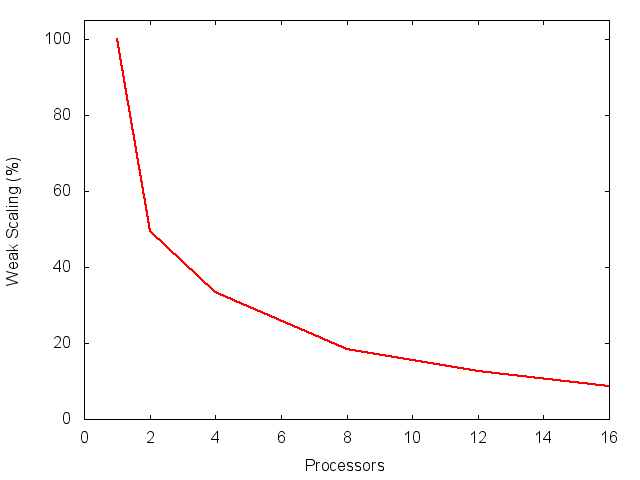
\includegraphics[width=0.7\columnwidth]{./fort_scaling/ws.png}
    		\caption{Weak scaling for simulations in Table~\ref{tab:ws} using the Fortran code parallelized with OpenMP.}
    		\label{fig:ws_fort_omp}
    	\end{center}
    \end{figure}
  
  \subsubsection{MPI}
  \textbf{Strong Scaling:}
  
  \textbf{Weak Scaling:}

	
  \section{Summary and Future Work}

\end{document}
